\documentclass[a4paper,10pt,fleqn]{article}
\usepackage{fullpage}
\setlength{\mathindent}{0pt}

% do not indent first line of paragraph.
\setlength{\parindent}{0cm}
% But separate them with 3-10mm
\setlength{\parskip}{6mm plus4mm minus3mm}

\usepackage[dutch]{babel}
\usepackage[utf8]{inputenc}

%~ \usepackage{fullpage}
%~ \usepackage[official]{eurosym} % depens on: texlive-fonts-recommended
\usepackage{amsmath}
\usepackage{amssymb}
%~ \usepackage{tabularx}

% Hyperref package, clickable internal links.
% colorlinks to remove ugly boxes around links...
% \usepackage[colorlinks]{hyperref}

\usepackage{enumerate}

\usepackage{subfigure}
\usepackage{pgf}
\usepackage{tikz}
\usetikzlibrary{arrows,automata}

\title{TI2736-A\\ Assignment 1:  Artificial Neural Network}

\author{
	David Akkerman - \\
	Jan Pieter Waagmeester - 1222848 \\
}

\begin{document}
\maketitle

\begin{enumerate}[1.]
	% 1. How many input neurons are needed for this assignment?
	\item Omdat er 10 eigenschappen zijn hebben we 10 inputneurons nodig.

	% 2. How many output neurons do you require?
	\item Voor de 7 verschillende classes hebben we 7 outputneurons nodig.

	% 3. How many hidden neurons will your network have? (Give an initial guess, later you will try different number of hidden neurons and analyze the network’s performance).
	\item We beginnen met 10 hidden neurons.

	% 4. Which activation function(s) will you use?
	\item We zullen de sigmoid-functie gebruiken:
	$$Y^{sigmoid} = \left( \frac{1}{1 + e^{-X}} \right)$$

	%5. Give a schematic diagram of your complete network
	\item Ons netwerk kan voorgesteld worden als in het volgende plaatje. Daarbij kan het aantal hidden neurons uiteraard gevarieerd worden. \\

	\begin{center}
		\tikzstyle{neuron}=[draw=black!50,minimum size=20pt,inner sep=3pt]
		\tikzstyle{input}=[rectangle]
		\tikzstyle{hidden}=[circle]
		\tikzstyle{output}=[circle]
		\tikzstyle{connection}=[draw=black!40, very thin]

		\begin{tikzpicture}[node distance=3cm,scale=1,auto]
			\def \scalar {0.9}

			\def \inputs {10}
			\def \hidden {10}
			\def \outputs {7}

			\foreach \m in {1,...,\inputs}{
				\node[neuron,input] (input-\m) at(0, {(-\m + \inputs / 2) * \scalar}) {$\m$};
			}

			\foreach \m in {1,...,\hidden}{
				\node[neuron,hidden] (hidden-\m) at(7, {(-\m + \hidden / 2) * \scalar}) {$\m$};
			}

			\foreach \m in {1,...,\outputs}{
				\node[neuron,output] (output-\m) at(14, {(-\m + \outputs / 2) * \scalar}) {$\m$};
			}

			% connections between neurons
			\foreach \j in {1,...,\hidden}{
				% input to hidden layer
				\foreach \i in {1,...,\inputs}{
					\path (input-\i) edge [connection] (hidden-\j);
				}
				% hidden to output layer
				\foreach \k in {1,...,\outputs}{
					\path (hidden-\j) edge [connection] (output-\k);
				}
			}


			% calculate the lowest Y of the three label positions and put each label there.
			\pgfmathparse{(-max(\inputs, \hidden, \outputs) / 2 - 1) * \scalar}
			\edef\labelY{\pgfmathresult}

			\node (input) 	at (0, \labelY)				{inputs};
			\node (wij)   	at (3.5, \labelY + 0.5)		{$w_{ij}$};
			\node (hidden)	at (7, \labelY)				{hidden};
			\node (wjk)		at (10.5, \labelY + 0.5)	{$w_{jk}$};
			\node (output) 	at (14, \labelY)			{outputs};
		\end{tikzpicture}
	\end{center}

    % 2.2 Training
	% 6. How and why did you divide your data into a training, validation and test set?
	\item We gebruiken ongeveer $50\%$ van de data voor training, $25\%$ voor validatie en $25\%$ als testset. De data lijkt aardig random gesorteerd te zijn, het is dus niet nodig om te zorgen dat er ongeveer even veel van elke class in elke set aanwezig is.

	% 7. How do you evaluate the performance of your network?
	\item Door te kijken naar de \textit{Mean square error} (MSE) op te trainingset, en op de validatieset.

	% 8. When and why do you decide to end the training?
	\item

	% 9. Train your network 10 times, each with different initial weights. How does the initialization impact the performance?
	\item

	% 2.3 Optimization
	% 10. Train your network with different amounts of hidden neurons. At least 3 times chosen within the range of 7-30 hidden neurons. Generate a plot of the final performance versus the number of hidden neurons in the network. (Hint: you can use the MATLAB command ❜boxplot' or 'errorbar' )
	\item

	% 11. Pick the architecture with the best result and show a plot of the performance of the training set and the validation set during training, across epochs.
	\item

	% 2.4 Evaluation
	% 12. What is the success rate of your network on the test set? How does it compare to the results of the validation set?
	\item

	% 13. Show a confusion matrix of your test set. How should it be read? Where did your network make the most mistakes? (Search for the meaning and purpose of a confusion matrix and use the function 'plotconfusion' from MATLAB).
	\item

	% 14. Feed the unknown set (provided on Blackboard) to the network. Export the resulting classes as a comma-separated file exactly as detailed in section 1.2.
	\item

	% 2.5 Matlab's Toolbox
	% 15. Use the Toolbox to create a network similar to the one you’ve just made. (You can start the toolbox GUI with 'nnstart' or directly go to pattern recognition with 'nprtool').
	\item Met \verb|nprtool| is het binnen een paar minuten mogelijk om een netwerk te maken wat er zo uitziet:

	\begin{figure}[!h]
		\centering
		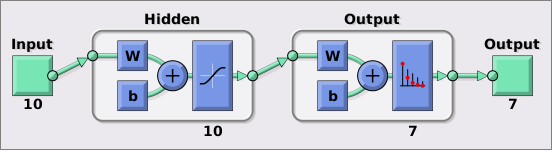
\includegraphics[width=.8\textwidth]{nprtool-diagram}
	\end{figure}

	% 16. Comment on the differences between your network’s performance and the Toolbox.
	\item De performance van dit netwerk is erg goed, en de training is ook erg snel klaar. Zelf met 10 hidden neurons worden succes-percentages van boven de $90\%$ gehaald.

	Tijdens het maken van het eigen neurale netwerk had ik het idee dat het gebruiken van de sigmoid-activatiefunctie wellicht voor de output-layer niet handig was. Dit netwerk gebruikt een softmax activatiefunctie in de output-layer.

	De veel hogere performance is waarschijnlijk verklaarbaar door bijvoorbeeld implementatie in correcte matrix-algebra en het toevoegen van het aanpassen van de \textit{learning rate}, het toevoegen van een momentum-term in de delta-rule (Negnevitsky, equation 6.17).
\end{enumerate}
\end{document}

